% !TEX root = ../thesis-example.tex
%
\section{Additional Camera Stencil}

When producing on small and / or amateur sets, there are usually constraints to 
size and proportions of the greenscreen production, thus limiting the 
recordable space. Since a calibrated playspace can be fetched from the SteamVR 
API to receive a proper-sized bounding box it is possible to do a projection of 
the greenscreens real size inside a virtual scene and use this as a stencil for 
the incoming video feed, effectively cropping off around all edges outside of a 
calibrated greenscreen.

A virtual projection can be seen in figure \ref{fig:stencil:projection} with 
reconstructed camera parameters. With help of the engine-editor a greenscreen 
can be calibrated and should match very closely to all real world parameters, 
allowing a real world camera to film over the edges of a greenscreen without 
destroying the image composition. If a VR actor is outside of the chroma key 
planes, the resulting image composition wouldn't be usable, thus this solution 
enhances a resulting image without major drawbacks.

\begin{figure}[htbp]
	\caption{Virtual projection and photo of VR actor - note: in-engine 
	screenshot and photos were taken shortly apart and therefore don't fit 
	exactly}
	\label{fig:stencil:projection}
	\begin{subfigure}[t]{.45\textwidth}
		\centering
		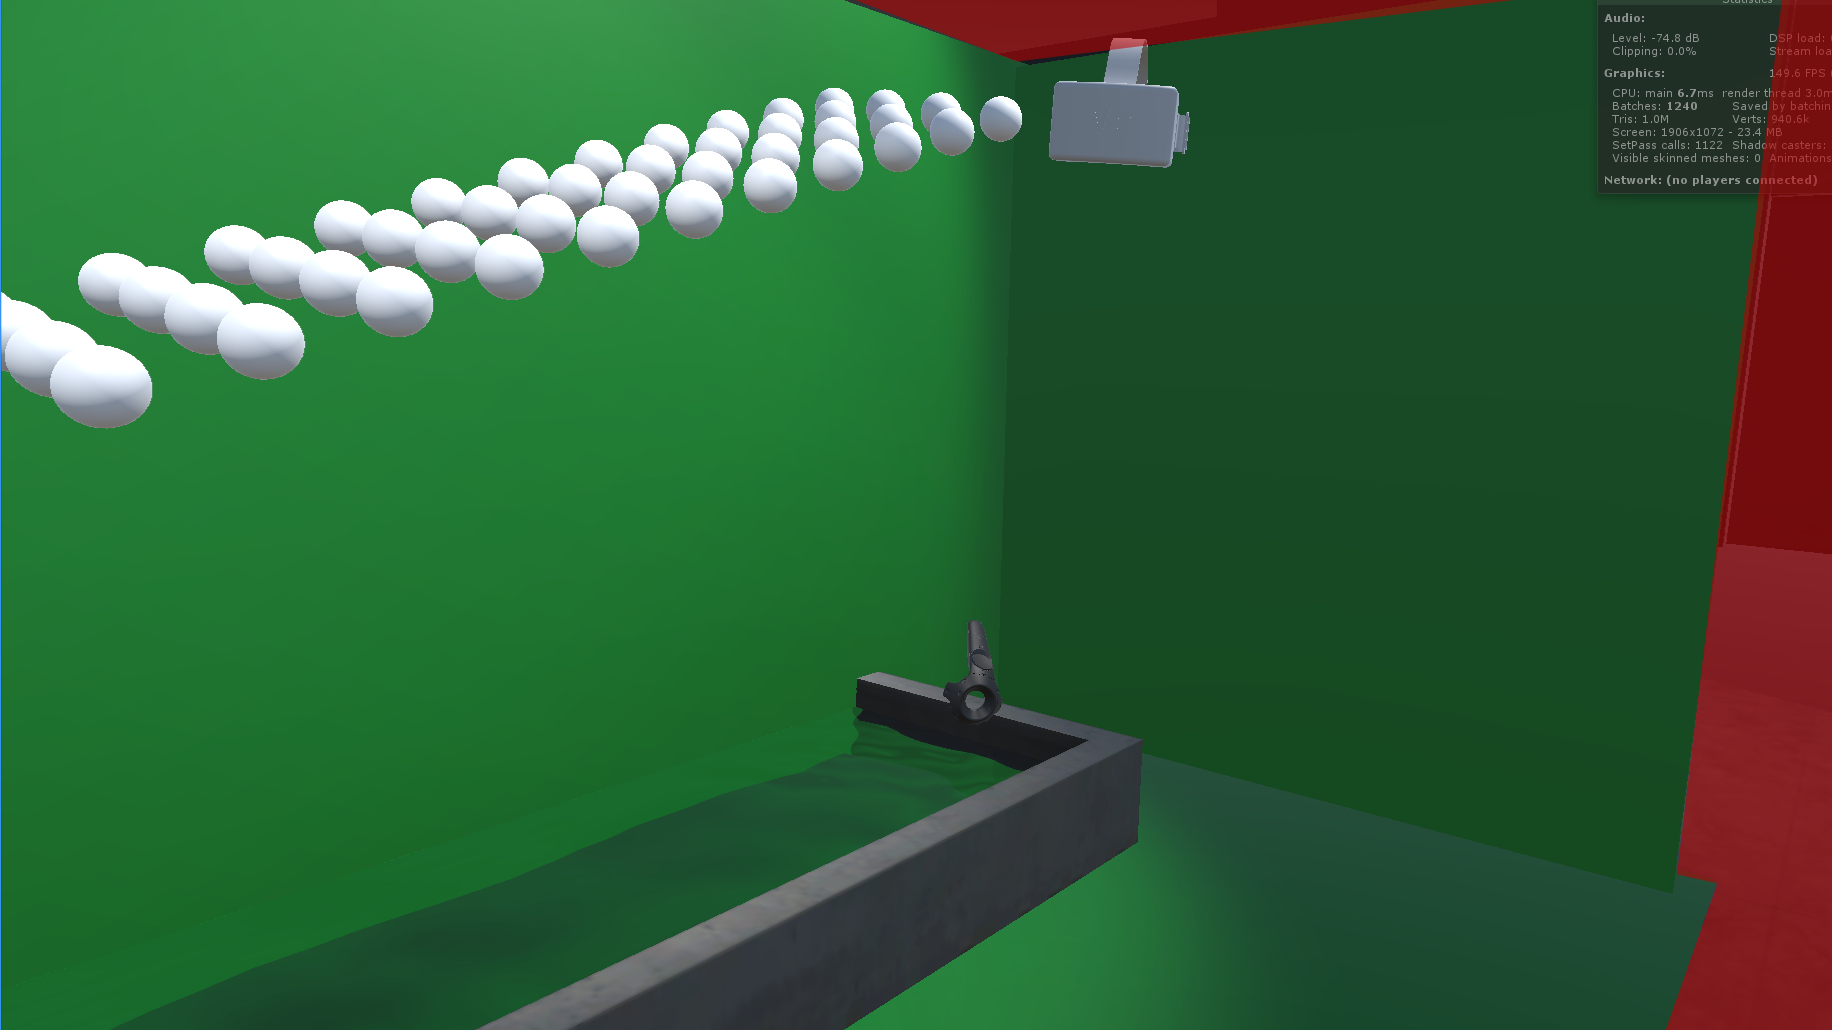
\includegraphics[width=\textwidth]{gfx/StencilProjection.png}
		\caption{Virtual reprojection of valid green screen - red colored areas 
		will be cut off}
	\end{subfigure}
	\begin{subfigure}[t]{.45\textwidth}
		\centering
		\includegraphics[width=\textwidth]{gfx/StencilCut.png}
		\caption{Masking what would be remaining video content - red colored 
		areas will be cut off}
	\end{subfigure}
\end{figure}

In-engine this setup is a simple addition: After registering another camera to 
the camera manager, it simply renders a green box. Taken from previous 
projection parameters in \ref{sec:projection-params} this virtual camera 
receives a dedicated culling mask which only contain all green box projection 
planes. All other cameras ignore this layer. After each drawn frame, Unity is 
able to clear the framebuffer with a color alpha as 0 - all remaining fragments 
from the green box write any color with an alpha as 1. This creates a lookup 
texture where an alpha-mask is created which will be transferred to the video 
feeds alpha.

Now we achieved a green box projection inside the same scene without using 
complex management processes with Unitys' scene manager. Due to the quick setup 
it works well for fast calibration and allows for a broad camera angle without 
degrading the mixed reality performance.
\newline
Unfortunately stencil-opertions are poorly documented in Unity and add an 
overhead which cannot be measured from builtin profiler tools - as such it adds 
unknown performance costs and have not been used in this thesis.